\section{Správa paměti, statické přidělování paměti, dynamické přidělování paměti, garbage collector, reprezentace informace v paměti.}
Každá paměť, která je přiřazena procesu se dělí na 4 základní bloky:
\begin{multicols}{2}
\begin{itemize}
    \item Segment instrukcí(Code)/Kódová oblast
    \item Datový segment(Data)/Datová oblast
    \item Halda/hromada(Heap)
    \item Zásobník(Stack)
    \vfill
\end{itemize}
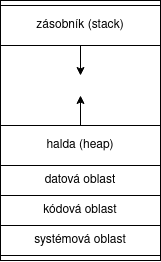
\includegraphics[scale=0.3]{BPC-TIN/images/pamet.png}
\end{multicols}
\textbf{Code}\,--\,je to množina strojových instrukcí, které naprosto jednoznačně provádí program. Dle těchto instrukcí PC postupuje ve výpočtu.

\textbf{Data}\,--\,v této části můžou být uložena data, která jsou známa při překladu programu (Hodnoty polí, konstant, proměnných, nějaké textové řetězce).

 Bloky Code a Data jsou známy v době překladu a jejich velikost se v průběhu nemění.

\textbf{Heap}\,--\,slouží k alokaci dynamické paměti. Je založena na stromové datové struktuře. Obsahuje objekty a instance proměnných(atributy třídy).

\textbf{Stack}\,--\,je důležitý pro volaní správných funkcí. Funguje na principu LIFO. Funguje tak že se ukládají funkce do stacku, se kterými se posunuje taktéž ukazatel na pozici v registeru tj. stack pointer. Po dokončení té funkce je odstraněna ze zásobníku a ukazatel změněn na předchozí funkci. Obsahuje metody/funkce, lokální proměnné a reference na proměnné. Video pro lepší vysvětlení \url{https://www.youtube.com/watch?v=uwV0hotRrLw}.\\

 Bloky Heap a Stack jsou dynamické a jejich velikost roste/se zmenšuje u každého jiným směrem v průběhu programu.

\begin{Large}\vspace{0,5cm} \textbf{Statické přidělování paměti}
\end{Large}

 Staticky se ukládají datové struktury, které jsou definovány při překladu programu. K jednotlivým paměťovým úsekům lze přistupovat pomocí názvu proměnné. V průběhu se adresa nemůže měnit.

\begin{Large}\vspace{0,5cm} \textbf{Dynamické přidělování paměti}
\end{Large}

 Dynamicky se paměť přiděluje na základě požadavku při průběhu programu. K dynamicky přidělenému paměťovému úseku se dá přistoupit pouze nepřímo pomocí ukazatele. Ukazatel je součástí statické nebo dynamické struktury. Dynamicky přidělovaná paměť se čerpá z vyhrazeného prostoru paměti počítače.

\begin{Large}\vspace{0,5cm} \textbf{Dynamické přidělování paměti bez regenerace}
\end{Large}

 Regenerace paměti je její pročištění od nepoužívaných částí paměti.

 Dynamické přidělovaní paměti bez regenerace přiděluje požadované úseky postupně tak jak jsou za sebou umístěny až do vyčerpaní vyhrazené paměti. Využívá pracovního ukazatele, který ukazuje na první adresu volné paměti. Nejčastěji pomocí operace "new" zapíše do paměti a změní ukazatel na novou hodnotu, která ukazuje na novou adresu volné části a v indikátoru paměti hodnotu obsazení označí true. Operace "free/delete" okamžitě neuvolní paměť, ale přepíše indikátor paměti na false. Kdy pak regenerace probíhá po větších částech. 

\begin{Large}\vspace{0,5cm} \textbf{Dynamické přidělování paměti s regenerací}
\end{Large}

 Na rozdíl od dynamického přidělovaní bez regenerací se zde regeneruje pro každé operaci "free/delete". S tím přichází problém s fragmentací paměti. Po uvolnění paměti by tyto části mohli vytvářet sekvence malých, oddělených a přitom sousedních prvků. Často je defragmentace těchto volných bloků spojena s operací "free/delete". Snaží se slučovat volné úseky se sousedními volnými úseky.

\begin{Large}\vspace{0,5cm} \textbf{Garbage collector}
\end{Large}

 Je nejpokročilejším způsobem dynamického přidělovaní paměti. Oproti předchozím způsobům je méně efektivní. 
Skládá se ze tří fází:
\begin{itemize}
    \item \textbf{Allocation}\,--\,přiděluje po sobě jdoucí úseky stejně jako metoda bez regenerace až do vyčerpání celého vyhrazeného prostoru.
    \item\textbf{Marking}\,--\,nastává pouze pokud je vyčerpán celý prostor. Prochází prostorem a vyhledává a označuje úseky, které nejsou aktivní a jejich návrat do společné paměti způsobí regeneraci.
    \item\textbf{Garbage collecting}\,--\,provádí se defragmentace přesunem všech uvolněných úseků do jednoho souvislého úseku. Tím se vytvoří nový souvislý úsek pro alokaci.
\end{itemize}

 Tyto tři fáze se opakují dokola, dokud nedojde k situaci, že nový úsek není dostačující pro fázi alokace. Z tohoto důvodu dojde k ukončení programu.

\vspace{1cm}
\textbf{Reprezentace informace v paměti}\,--\,pokud je datový typ primitivní je uložen na přímo v paměti a u objektů je reprezentován pouze ukazatelem na místo v paměti.\footnote{Pokud si to nedokážete představit, tak například jeden \textit{integer} jednoduše zabere v paměti 32bitů. Zatímco \textit{objekt} (v C si lze představit jako \textit{struct}) obsahující dva integery, bude v paměti reprezentován jako \textit{odkaz} (pointer) na tu část paměti kde začíná první integer. (nedá se úplně s jistotou říct, že zabere 64bitů, jelikož se zpravidla dodá padding pro metadata)} 







\newpage
\section{Jazyk UML a objektově orientovaný návrh - dědičnost, generalizace, asociace 1:n, n:1, n:n, agregace a kompozice.}

 \textbf{Jazyk UML} je grafický jazyk pro popis programových systémů. Slouží pro vizualizaci, specifikaci, návrh a dokumentaci systémů. K zobrazení se využívají diagramy, kde nejčastěji používané jsou:
\begin{enumerate}
    \item Strukturální
    \begin{enumerate}
        \item Diagram tříd
        \item Diagram případů užití
        \item Diagram komponent
        \item Diagram nasazení
    \end{enumerate}
    \item Behaviorální
    \begin{enumerate}
        \item Diagram aktivit
        \item Diagram sekvencí
        \item Diagram stavů.
    \end{enumerate}
\end{enumerate}
Nejpoužívanější jsou diagramy tříd a případů užití. Diagram tříd popisuje strukturu systému, znázorňuje datové struktury a operace u objektů a souvislosti mezi nimi. Skládá se z tříd, rozhraní, abstraktních tříd. Tyto tři prvky se dále skládají z názvu třídy/rozhraní, atributů (rozhraní neobsahuje atributy), a operace (metody/funkce) Diagram případů užití se nejčastěji používá při komunikaci se zákazníkem a méně technicky znalou stranou. Skládá se z herců (actor) a případů užití a systém. Tyto strany jsou propojeny jak mezi sebou tak i sami se sebou pomocí těchto propojení\,--\,asociace, generalizace, rozšíření vztahu, vztah zahrnuje

\textbf{Objektově orientovaný návrh} je jeden ze způsobů jak reprezentovat informaci. Vychází z principů reálného světa, neboli je jednoduše srozumitelný pro člověka. Není spojen s žádným programovacím jazykem ale jazyk, který bude použit pro implementaci musí splňovat objektově orientované principy. Výhodou OO návrhu může být, že při návrhu lze určit co jaká část programu komunikuje z jakou a co každá dělá, takže se sníží počet chyb v kódu a tím i náklady. OO návrh se nezabývá konkrétní implementací ale pouze vazbami mezi objekty.

Kdy není vhodný OO přístup? Není vhodné ho použít jestliže na cílové platformě neexistuje překladač OO jazyka. Nebo potřebuji to v jazyce, který nepodporuje OOP. Přepis stávající kódu by byl neekonomický, hlavně u projektů s krátkou životností.

\begin{Large}\vspace{0,5cm} \textbf{Vztahy mezi třídami}
\end{Large}

\textbf{Závislost}\,--\, je dynamický a zároveň nejslabší vztah. Ukazuje jak co na sobě závisí.\\
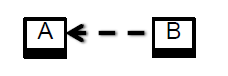
\includegraphics[scale=1]{BPC-TIN/images/zavislost.PNG}

\textbf{Asociace}\,--\, je pevný vztah. Určuje vztah mezi dvěma prvky, které mohou existovat nezávisle na sobě. Asociace může mít směr od jednoho prvku k druhému nebo obousměrně. Objekt ve směru šipky může nalézt odkaz na následujíc objekty. \\
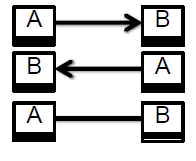
\includegraphics[scale=1]{BPC-TIN/images/asociace.PNG}

\textbf{Násobnost asociací}\,--\, určuje kolik vazeb může mít danný objekt. Například 1:n může být 1 objekt a ten mít reference na n objektů ke kterým má asociaci (faktura:n * položka).

\textbf{Agregace}\,--\, je typ asociace. reprezentuje vztah typu celek--část. Zde je u celku umístěn kosočtverec. Celek je entita, která drží kolekci prvků. Část může existovat bez celku nebo být součástí jiných kolekcí. \\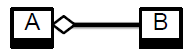
\includegraphics[scale=1]{BPC-TIN/images/agregace.PNG}

\textbf{Kompozice}\,--\, je typ asociace. Je to nejsilnější vztah a je podobná agregaci. S rozdílem v tom že část nemá bez celku smysl. pokud zanikne celek zaniknou i části. U celku je násobnost vždy 1.\\ 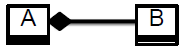
\includegraphics[scale=1]{BPC-TIN/images/kompozice.PNG}

\textbf{Dědičnost/generalizace}\,--\,se využívá jestliže mají některé třídy společné vlastnosti. Tím například nemusíme vytvářet duplicitní kód. Směr šipky udává od koho třída dědí (obrázek b dědí z a). Díky tomuto lze jednodušeji rozšířit třídu o atributy a operace. Neplést si z asociací nijak nesouvisí.\\
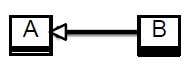
\includegraphics[scale=1]{BPC-TIN/images/dedicnost.PNG}






\newpage
\section{Třídy složitosti paměťové a časové. Notace Theta. Notace Omega. Notace velké-O. Asymptotický popis složitosti algoritmu. Posouzení složitosti známých algoritmů řazení. Posouzení složitosti algoritmu vyhledávání. Srovnání lineárních a nelineárních struktur. Vztah časové a paměťové složitosti.}

Složitost je vztah algoritmu k prostředkům (čas a velikost paměti). Paměťová složitost je závislost paměťových nároků na vstupních datech. Zatímco časová je dána hrubým odhadem počtu kroků, který daný algoritmus musí provést na základě délky vstupních dat.

\begin{Large}\vspace{0,5cm} \textbf{Asymptotická složitost}
\end{Large}

Jelikož ne vždy lze určit přesnou složitost algoritmu tak byla vyvinuta asymptotická složitost. Tato složitost aproximuje chovaní funkce ze tří pohledu:
\begin{itemize}
    \item Nejlepší případ $\Omega$ (Omega)\,--\,značí spodní hranici trvání algoritmu.
    \item Průměrný případ $\Theta$ (Theta)\,--\,odhaduje nejpravděpodobnější dobu trvání algoritmu.
    \item Nejhorší případ notace O (Omicron, big-O)\,--\,značí horní hranici trvání algoritmu. Je nejčastěji používaná.
\end{itemize}

\begin{table}[h]
    \begin{tabularx}{\textwidth}{|c|c|X|}\hline
        Konstantní & O(1) & Nezávisí na velikosti vstupních dat\\\hline
        Logaritmická & O($\log{n}$) & Počet operací odpovídá logaritmu např. vstup 1\,000\,000\,000 $==$ 30 operací\\\hline
        Lineární & O($n$)& počet operací je závislý na velikosti vstupních dat\\\hline
        Kvazilineární& O($n\log{n}$)& Zástupce quicksort\\\hline
        Kvadratická& O($n^2$)& Např 500 vstupů $==$ 250\,000 operací\\\hline
        Kubická & O($n^3$)& Např. 200 vstupů $==$ 8\,000\,000 operací\\\hline
        Exponenciální&O($2^n$)& Exponenciální růst počtu operací\\\hline
        Faktoriální&O($n!$)& Faktoriální růst počtu operací\\\hline
    \end{tabularx}
\end{table}

\textbf{Polynomiální algoritmy}\,--\,Jsou takové algoritmy jejichž notace v big-O je ohraničena polynomiální funkcí shora. Spadají zde například $\log{n}$, $k*n$, $3n^3 + 4n$, $2*n\log{n}$ a podobné. Nepatří sem exponenciální, faktoriální a jim podobné. Abychom algoritmus označili jako efektivní jeho vykonání by mělo být možné v polynomiálním čase jinak ho lze označit jako neefektivní. Při vysokých hodnotách v kryptografii by ne-polynomiální algoritmy byli nepoužitelné.

\begin{Large}\vspace{0,5cm} \textbf{Algoritmy řazení.}
\end{Large}

Třídění pomocí algoritmů Bubble Sort, Insert Sort a Select Sort má složitost O($n^2$). Algoritmus Quick Sort má složitost $\theta$($n\log{n}$), kdy v nejhorším případě může nabývat až O($n^2$). Algoritmus Merge Sort má složitost O($n\log{n}$).

\vspace{1cm}
\begin{Large}\vspace{0,5cm} \textbf{Algoritmy hledání.}
\end{Large}

Dva základní algoritmy pro hledání jsou \textit{Binary search}\footnote{Funguje na principu půlení seřazeného seznamu, pokud je hledaná hodnota v půlce tak skončí, pokud je menší tak půlí levou stranu a pokud větší tak pravou. Takto iteruje dokud nenajde číslo. Více:  \url{https://en.wikipedia.org/wiki/Binary_search_algorithm}} a \textit{Linear search}\footnote{Linear search je naprosto jednoduchý lineární průchod seznamem, kde se postupně hledá požadovaná hodnota. Alternativa je Linear Sentinel search, která přidá hledanou hodnotu na konec seznamu. Více: \url{https://www.geeksforgeeks.org/linear-search/} \url{https://algorithmoftheweek.blog/2020/06/10/sentinel-linear-search/}} . \textit{Binary} funguje lépe než, \textit{Linear} ale pouze pro větší seznamy, zároveň je třeba předem seznam seřadit. \\

\textbf{Složitosti (Big-O):}

\begin{table}[h]
    \centering
    \begin{tabular}{|c|c|c|}\hline
         Algoritmus & Časová & Paměťová\\\hline
         Linear Search & O($n$) & O($1$)\\\hline
         Binary Search & O($\log n$) & O($1$)\\\hline
    \end{tabular}
\end{table}


\vspace{1cm}
\begin{Large}\vspace{0,5cm} \textbf{Lineární a nelineární struktury.}
\end{Large}

\textbf{Lineární}\,--\,zde spadají pole, seznamy, zásobník, fronta.
\begin{table}[h]
    \centering
    \begin{tabular}{|c|c|c|c|c|}\hline
         Struktura & Přidat & Vyhledat & Smazat & Výběr dle indexu\\\hline
         Pole & O($n$) & O($n$) & O($n$) & O($1$) \\\hline
         Seznam & O($1$) & O($n$) & O($n$) & O($n$)\\\hline
         Pole proměnlivé délky & O($1$) & O($n$) & O($n$) & O($1$) \\\hline
         Zásobník & O($1$) & -- & O($1$) & -- \\\hline
         Fronta & O($1$) & -- & O($1$) & -- \\\hline
    \end{tabular}
\end{table}

\textbf{Nelineární}\,--\,zde můžou spadat stromy, které pokud jsou nějak vyvažovány, tak mají náročnost O($\log{n}$). Pokud se nevyvažují tak náročnost je O($n$).

\begin{Large}\vspace{0,5cm} \textbf{Vztah časové a paměťové složitosti.}
\end{Large}

Většina algoritmů je kompromisem mezi těmito dvěma druhy složitosti. Pokud bychom měli algoritmus s vysokými nároky na časovou složitost (aby byl co nejrychlejší) tak jeho paměťová složitost bude vzrůstat. Většinu algoritmů je nějakým způsobem optimalizovaná nebo ji lze optimalizovat.

\newpage

\begin{Large}\vspace{0,5cm} \textbf{Třídy složitosti}
\end{Large}

Vyjadřuje jak náročný je výpočet je nezbytný k vyřešení problému.\\
Rozdělení:
\begin{itemize}
    \item Třída P\,--\,schůdné algoritmy. Jsou proveditelné v polynomiálním čase na deterministickém turingově stroji.
    \item Třída NP\,--\,neschůdné algoritmy. Je možné je provést v polynomiálním čase na \textbf{nedeterministickém} TS (nebyl doposud sestaven). Spadají pod ně i všechny algoritmy z třídy P
    \item Třída NP-těžké\,--\,přinejmenším tak těžké, jako nejtěžší z NP. Nemusí být vykonatelné pomocí TS.
\end{itemize}









\newpage
\section{Abstraktní datový typ (ADT). ADT lineární seznam. ADT cyklický seznam. Operace vkládání, mazání a~vyhledávání prvku v ADT lineární seznam. ADT zásobník, ADT fronta.}

Abstraktní datový typ je množina druhů dat (hodnot) a příslušných operací, které jsou přesně specifikovány a to nezávisle na konkrétní implementaci. Zjednodušeně ADT je reprezentováno rozhraním, kde uživatele tohoto rozhraní zajímá pouze, jak se používá a ne jak je implementováno. Poté co je konkrétní ADT implementován v programovacím jazyce stává se z něj datová struktura.

ADT dělíme podle počtu datových položek na statický a dynamický datový typ. Statický datový typ má neměnnou velikost a dynamický mění velikost dle provedené operace. Dále se dělí jestli mají jednoznačného bezprostředního následníka na lineární a nelineární. Lineární mají následníka a u nelineárních neexistuje přímý jednoznačný následník.

\textbf{Dělení ADT:}
\begin{itemize}
    \item Lineární
    \begin{itemize}
        \item Pole\,--\,statický
        \item Seznam\,--\,dynamický
        \item Zásobník\,--\,dynamický
        \item Fronta\,--\,dynamický
    \end{itemize}
    \item Nelineární
    \begin{itemize}
        \item Strom\,--\,dynamický
        \item Množina (Set)\,--\,dynamický
    \end{itemize}
\end{itemize}

\begin{Large}\vspace{0,5cm} \textbf{Lineární seznam}
\end{Large}

ADT lineární seznam je seznam, kde každý uzel má unikátního následníka.
Výhodou lineárního seznamu je že má efektivní vkládání a mazání ale neefektivní přístup k prvkům. Na rozdíl od pole, kde je rychlá indexace prvků. Každý prvek obsahuje data a ukazatel na další prvek v seznamu.
\begin{center}
    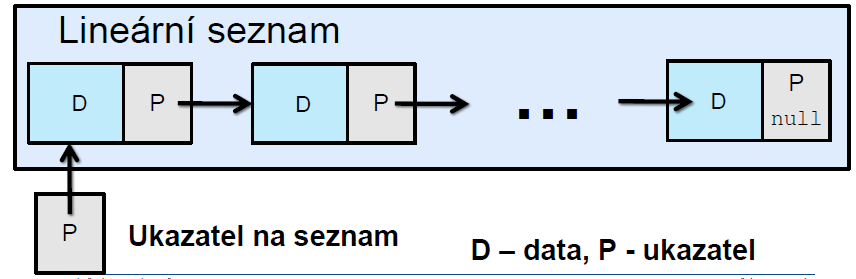
\includegraphics[scale=0.5]{BPC-TIN/images/linsez.PNG}
\end{center}

Možné operace s ADT seznamem:
\begin{itemize}
    \item Nalezení délky N seznamu
    \item Výpis všech prvků seznamu
    \item Vytvoření prázdného seznamu
    \item Získaní k-tého prvku ze seznamu
    \item Vložení novéhé prvku za k-tý prvek seznamu
    \item Smazaní prvku ze seznamu
    \item Nalezení následujícího prvku za aktuálním v seznamu
    \item Nalezení předchozího prvku před aktuálním v seznamu
\end{itemize}

\textbf{Cyklický lineární seznam}\,--\,stejný jako lineární ale poslední prvek nemá ukazatel null ale odkaz na první prvek seznamu.

\begin{center}
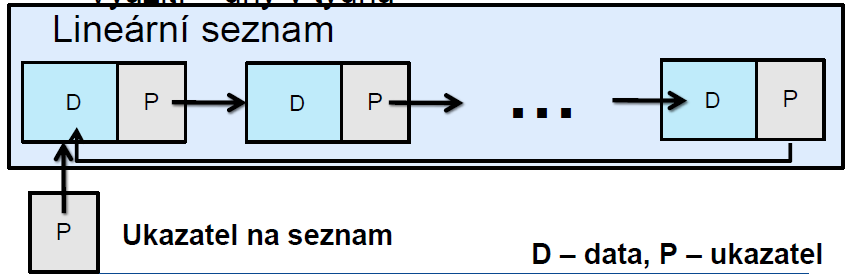
\includegraphics[scale=0.5]{BPC-TIN/images/cycsez.PNG}
\end{center}

\textbf{Obousměrně vázaný lineární seznam}\,--\,nemá pouze ukazatel na další prvek ale i na předchozí. Umožňuje procházení v obou směrech.

\begin{center}
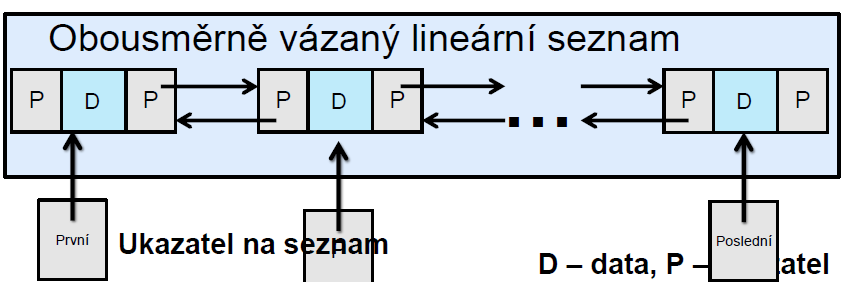
\includegraphics[scale=0.5]{BPC-TIN/images/obousez.PNG}
\end{center}

\textbf{Vkládaní do lineárního seznamu}\,--\,vložit prvek na určitou pozici funguje tak, že se najde pozice k kde se zde vloží prvek který bude odkazovat na prvek, který byl předtím na pozici k a v prvku k-1 se přepíše ukazatel na nový prvek. Operace fungují stejně jen jsou vázány na obě strany.

\begin{center}
    
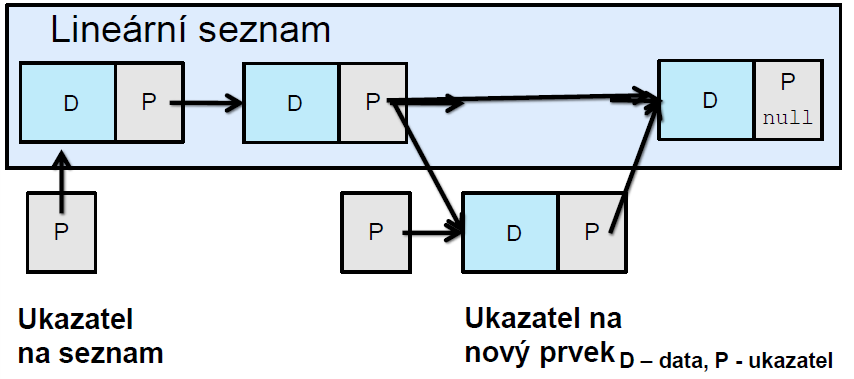
\includegraphics[scale=0.5]{BPC-TIN/images/sezins.PNG}
\end{center}

Pokud vkládáme na začátek tak se přepisuje ukazatel pole na první prvek a ve vkládaném prvku se přidá ukazatel na předchozí první prvek.

\begin{center}
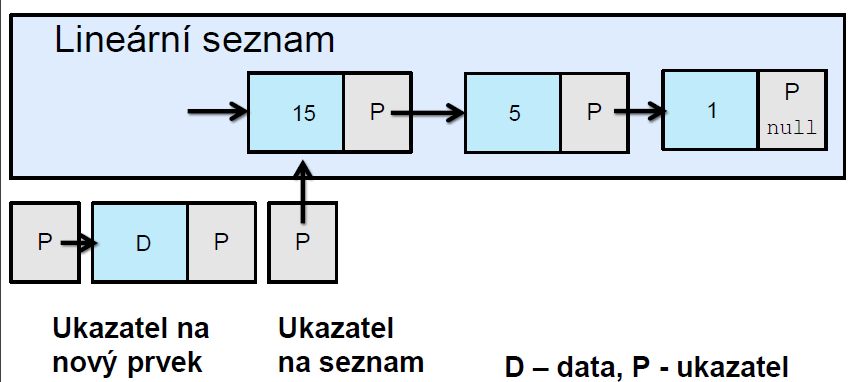
\includegraphics[scale=0.5]{BPC-TIN/images/sezinsfirst.PNG}

\vspace{1cm}
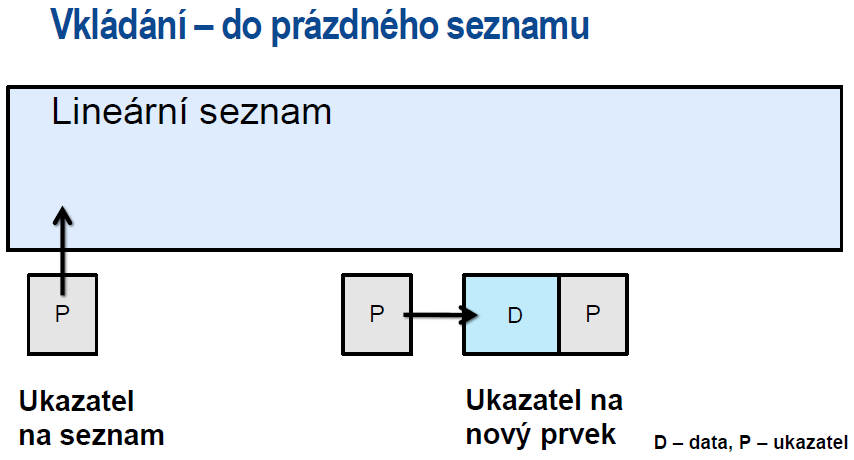
\includegraphics[scale=0.5]{BPC-TIN/images/sezinsempty.PNG}
\end{center}

\textbf{Mazaní v lineárním seznamu}\,--\,mazaní prvku na pozici k funguje tak že prvek k-1 přepíše ukazatel na prvek k+1. U prvního prvku se přepíše pouze ukazatel na další prvek.
\begin{center}
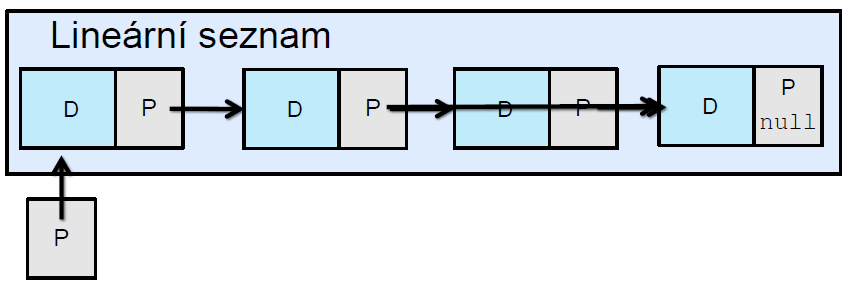
\includegraphics[scale=0.5]{BPC-TIN/images/sezdel.PNG}
\end{center}

\textbf{Vyhledávaní v lineárním seznamu}\,--\,dá se vyhledávat podle prvku nebo podle dat. Pomalu iteruje seznamem dokud nenarazí na ten prvek nebo konec seznamu. U obousměrného se dá hledat od začátku a od konce.

\begin{Large}\vspace{0,5cm} \textbf{Zásobník}
\end{Large}

Je dynamická datová struktura umožnující vkládaní a odebírání hodnot tak, že naposledy vložená hodnota se odebere jako první (LIFO). Základní operace jsou Vložený na vrchol, odebraní z vrcholu a test na prázdnost zásobníku. 

\begin{Large}\vspace{0,5cm} \textbf{Fronta}
\end{Large}

Je dynamická datová struktura, kde se odebírají prvky v tom pořadí v jakém byli vloženy (FIFO). Základní operace jsou stejné jako u zásobníku. Existuje tzv. prioritní fronta, která funguje na principu fronty ale bere z ní podle priority.








\newpage
\section{Abstraktní datový typ strom. Abstraktní datový typ binární strom. Úplný binární strom. Abstraktní datový typ binární vyhledávací strom (operace vložení, odstranění, smazání uzlu stromu).}

\textbf{ADS typu strom}\,--\,je nelineární dynamická abstraktní datová struktura. Každý uzel stromu může mít n potomků a zároveň má pouze jednoho předchůdce. Nejčastější zástupci jsou obecný strom nebo n-ární strom. Rozdíl je v tom, že n-ární má maximální počet potomků rovný n. Skládá se z uzlů, které se pojmenovávají:
\begin{itemize}
    \item Kořenu\,--\,existuje pouze jeden. Je to uzel bez předchůdce.
    \item List\,--\,jsou to uzly, které nemají následníka
    \item Vnitřní uzel\,--\,jsou to uzly které nejsou kořenem ani listem stromu.
\end{itemize}
\begin{center}
    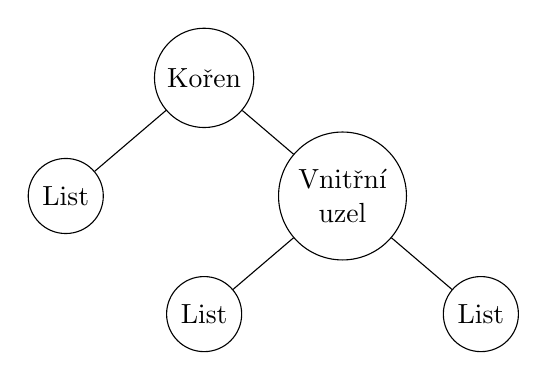
\begin{tikzpicture}[sibling distance=10em,
  every node/.style = {shape=circle,
    draw, align=center,
    top color=white, bottom color=white}]]
  \node {Kořen}
    child { node {List} }
    child { node {Vnitřní\\uzel}
      child { node {List}}
      child { node {List} } };
\end{tikzpicture}
\end{center}

\begin{Large}\vspace{0,5cm} \textbf{Binarní strom}
\end{Large}

Binární strom je strom, který má nanejvýše 2 potomky na jeden uzel.

Za \textbf{Úplný binární strom} se považuje binární strom, který se plní po úrovni hloubky z levé strany. Dokud není plně zaplněn levý potomek tak se neplné pravý. Hezká ukázka zde \url{https://home.cs.colorado.edu/~main/supplements/pdf/notes10a.pdf}

\begin{Large}\vspace{0,5cm} \textbf{Binarní vyhledávací stromy}
\end{Large}

U těchto stromů musí platit, že levá část potomků musí být vždy menší než kořen a pravá část vždy vetší. Tzn. prvky jsou seřazeny. Tyto stromy mohou být nevyvážené ale častěji se také vyvažují, aby bylo dosaženo jejich optimální složitosti O($\log{n}$). Mohl by totiž nastat případ, kdy by ze stromu vznikl pouze strom.
\begin{multicols}{2}
\begin{center}
Vyvážený strom
    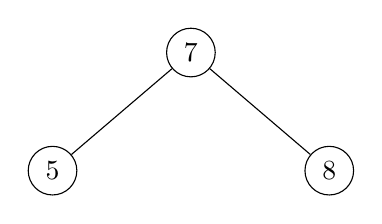
\begin{tikzpicture}[sibling distance=10em,
  every node/.style = {shape=circle,
    draw, align=center,
    top color=white, bottom color=white}]]
  \node {7}
    child { node {5} }
    child { node {8}};
\end{tikzpicture}

\vspace{3cm}
Nevyvážený strom


    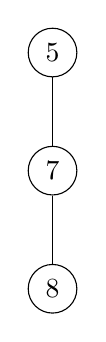
\begin{tikzpicture}[sibling distance=10em,
  every node/.style = {shape=circle,
    draw, align=center,
    top color=white, bottom color=white}]]
  \node {5}
    child { node {7}
      child { node {8} } };
\end{tikzpicture}
\end{center}
\end{multicols}
U nevyvážené stromu lze vidět, že by se jednalo spíše o seznam. U vyvážených bin stromů by rozdíl hloubky levé a pravé části měl být 0 nebo 1.

\textbf{Vyhledávaní v binárních vyvážených stromech}\,--\,postupuje se od kořene směrem dolů, kde se porovnává jestli prvek bude v levém nebo pravém uzlu pokud to už není námi hledaný prvek. Tak se postupuje vždy na každém navštíveném uzly dokud nenajdeme hledanou hodnotu nebo konec uzlu. Při hledání min/max se vždy vydáme do leva/prava dokud nenarazíme na uzel, který má svůj levý/pravý uzel roven null.

\textbf{Vložení do binárních stromů}\,--\,postupujeme stejně jako při vyhledávaní jen z rozdílem toho, že vkládáme až najdeme hodnotu null nebo úplně stejnou položku v tom případě záleží, jak se s tím v implementaci poradíme (přepíšeme/nepřepíšeme).

\textbf{Odstranění prvků}\,--\,nemají žádného potomka, má jednoho potomka, má dva potomky.

\textbf{Nemají potomka}\,--\,uzel se pouze odstraní a z jeho rodiče se smaže reference na něj.

\textbf{Mají jednoho potomka}\,--\,máme-li uzel tak jeho rodič zamění referenci toho uzlu za referenci potomka.

\textbf{Mají dva potomka}\,--\,dvě varianty. Buď pravého prvku (PL) nebo levého prvku (LP).\\
Pro pravý prvek to bude nalezneme uzel, který je nejvíc napravo v levém stromu a ten zaměníme za uzel, který chceme smazat. Takže nejpravější uzel v levém stromu převezme referenci z mazaného uzlu a rodič mazaného uzlu změní referenci na nejpravější uzel levého stromu. \\
Pro levý prvek je to podobné jen se vybírá nejlevější uzel z pravého stromu. Viz obrázky.

PL
\begin{center}
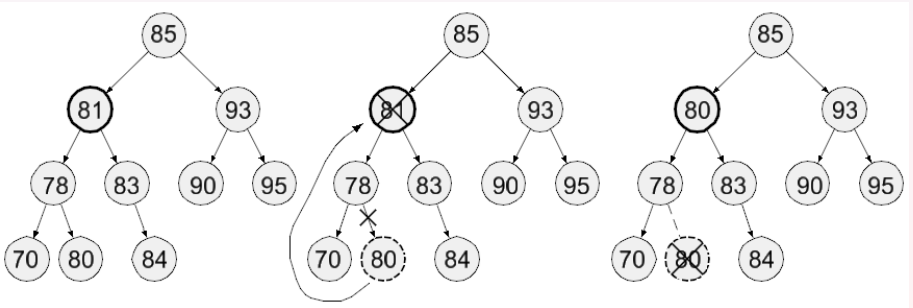
\includegraphics[scale=0.8]{BPC-TIN/images/treePL.PNG}
\end{center}

LP
\begin{center}
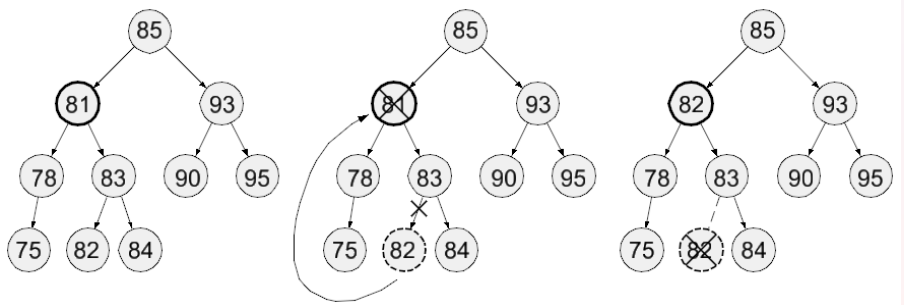
\includegraphics[scale=0.8]{BPC-TIN/images/treeLP.PNG}
\end{center}




\newpage
\section{Průchody stromy in-order, pre-order, post-order.}
\textbf{Pre-order}\,--\,nejprve se zpracuje kořen, poté levý podstrom a nakonec pravý podstrom. Využívá se k vytvoření kopie stromu. Tak aby vypadal stejně.
\begin{center}
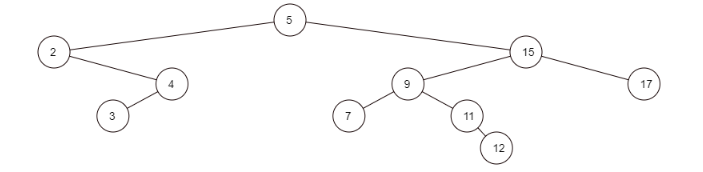
\includegraphics[scale=1]{BPC-TIN/images/tree.PNG}
\end{center}
Čtení pomocí pre-order bude posloupnost 5, 2, 4, 3, 15, 9, 7, 11, 12, 17.

\textbf{In-order}\,--\,nejprve se zpracuje levý podstrom poté kořen a nakonec pravý podstrom. Výsledkem je v příkladu čísel posloupnost od nejmenšího k největšímu. Využívá se k získaní popořadě jdoucích hodnot závislých tak jak máme vytvořen komparátor.
\begin{center}
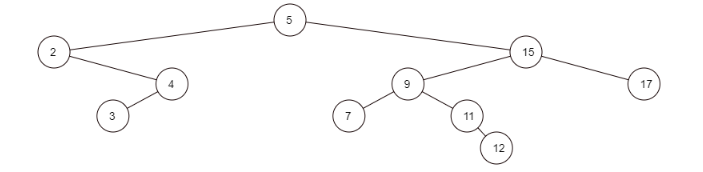
\includegraphics[scale=1]{BPC-TIN/images/tree.PNG}
\end{center}
Čtení pomocí in-order bude posloupnost 2, 3, 4, 5, 7, 9, 11, 12, 15, 17.

\textbf{Post-order}\,--\,nejprve se zpracuje levý podstrom poté pravý a nakonec kořen. Využívá se k mazání stromu od listů ke kořenu.
\begin{center}
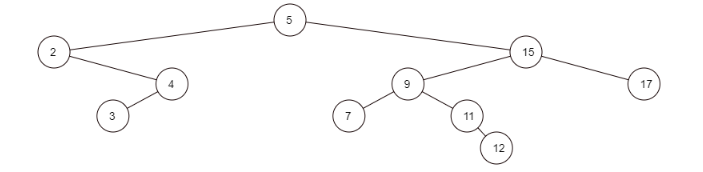
\includegraphics[scale=1]{BPC-TIN/images/tree.PNG}
\end{center}
Čtení pomocí post-order bude posloupnost 3, 4, 2, 7, 12, 11, 9, 17, 15, 5.














\newpage
\section[Problematika nevyvážených stromů. Vyvažování stromů AVL - rotace: jednoduchá levá, jednoduchá pravá, dvojitá levá, dvojitá pravá. Red-Black stromy. Posouzení z pohledu časové a paměťové složitosti. ADT hashovací tabulky. Řešení kolizí hashovacích tabulek. Srovnání výkonnosti binárních vyhledávacích stromů a hashovacích tabulek.]{Problematika nevyvážených stromů. Vyvažování stro-mů AVL - rotace: jednoduchá levá, jednoduchá pravá, dvojitá levá, dvojitá pravá. Red-Black stromy. Posouzení z pohledu časové a paměťové složitosti. ADT hashovací tabulky. Řešení kolizí hashovacích tabulek. Srovnání výkonnosti binárních vyhledávacích stro-mů a hashovacích tabulek.}

Nevyvážený strom je problematický v tom, že jeho složitost může klesnout až na O($n$) z O($\log{n}$). Z tohoto důvodu má smysl stromy vyvažovat.

Vyvážený strom má hloubku levého a pravého podstromu rovnou vždy 0 nebo 1. Pokud má hloubku větší tak se označuje za nevyvážený a z pohledu problematiky by se měl vyvážit například metodou AVL nebo Red-Black stromy.

\begin{Large}\vspace{0,5cm} \textbf{Vyvažování}
\end{Large}

\textbf{AVL stromy}\,--\,mají výhodu v tom, že jsou dobře vyvážené ale hrozí zde problém mnohonásobné rotace. Takže vkládání může být méně efektivní. Mají velice efektivní vyhledávání.

Vyvažuje se dvěma typy rotace, u kterých pak dále rozlišujeme stranu. Vizualizace \url{https://www.cs.usfca.edu/~galles/visualization/AVLtree.html}

\textbf{Red-Black stromy}\,--\,nejsou tak dobře vyvážené jako AVL, ale řeší problém mnohonásobné rotace. Efektivní vkládání, ale méně efektivní vyhledávání.

Při vyvažování platí pravidla:
\begin{itemize}
    \item Každý uzel je červený nebo černý.
    \item Kořen je vždy černý.
    \item Všechny listy jsou černé.
    \item Potomci červeného jsou vždy černí.
    \item Každá cesta z libovolného uzlu do jeho podřízených listů obsahuje stejný počet černých uzlů.
\end{itemize}
Vizualizace \url{https://www.cs.usfca.edu/~galles/visualization/RedBlack.html}


\begin{Large}\vspace{0,5cm} \textbf{Hashovací tabulka}
\end{Large}

Hashovací tabulka spojuje klíč s odpovídající hodnotou. Klíč je vypočítán z obsahu položky tak aby byl klíč co nejjednoznačnější a nedocházelo ke kolizím, vše vychází z pravděpodobnosti o hashovacích funkcích. Využívají se nejčastěji v databázích nebo k rychlému vyhledávaní v polích.

\textbf{Vkládání}\,--\,Z vkládaného prvku se se udělá hash. Tento hash se přiřadí do pole, na místo, které mu odpovídá. Jestliže je místo obsazeno přiřadíme mu další volné místo dle algoritmu.

\textbf{Vkládání}\,--\,Při vyhledávání využijeme klíče, který nám vrátí index položky. Jestliže na odpovídajícím indexu se nenachází daná položka tak pomocí algoritmu vypočteme, kde je další místo, kde se položka může nacházet.

\begin{Large}\vspace{0,5cm} \textbf{Hashovací tabulka\,--\,řešení kolizí}
\end{Large}

\textbf{Řetězení tabulek}\,--\,pokud dojde ke kolizi vložíme prvky do lineárního seznamu za sebe.

\textbf{Otevřené adresování linear probing}\,--\,pokud dojde ke kolizi, tak prvek vkládáme na další možné volné místo. Zde si musíme hlídat, aby se tabulka celá nenaplnila.

\textbf{Otevřené adresování double hashing}\,--\,podobné linear probing jen se neposunujeme na další volné místo ale hashujeme dále.

\begin{Large}\vspace{0,5cm} \textbf{Hashovací tabulka vs binární strom}
\end{Large}

Hashovací tabulka je rychlejší na vyhledávání pokud je dobře napsána hashovací funkce ve špatném případě lze dojít k O(n). Nevýhoda je, že nelze vyhledávat pokud máme jen částečný klíč nebo potřebujeme v nějakém intervalu. Další nevýhodou je složitost vytvoření hashovacích tabulek oproti stromu.










\newpage
\section{Jednoduché a pokročilejší řadící techniky a jejich srovnání. Stabilita řadícího algoritmu. Bubble sort. Insertion sort. Selection sort. Shell sort. Merge sort. Heap sort. Quick sort.}

\begin{Large}\vspace{0,5cm} \textbf{Typy řazení}
\end{Large}

\textbf{Řazení výběrem}\,--\,najde se vždy nejmenší se zbývajících prvků a uloží se na konec už seřazených.

\textbf{Řazení vkládáním}\,--\,z neseřazené množiny se postupně bere prvek po prvku a vkládá se na správné místo přičemž začáteční množina už seřazených je prázdná.

\textbf{Řazení záměnou}\,--\,v množině najdeme vždy dvojici, která je ve špatném pořadí a přehodíme ji.

\textbf{Řazení slučováním}\,--\,vstupní množinu rozdělíme na části, které se seřadí. Tyto seřazené části se poté sloučí takovým způsobem aby byli seřazené.

\begin{Large}\vspace{0,5cm} \textbf{Porovnání algoritmů}
\end{Large}

Třídění pomocí algoritmů Bubble Sort, Insert Sort a Select Sort má složitost O($n^2$). Algoritmus Quick Sort má složitost $\theta$($n\log{n}$), kdy v nejhorším případě může nabývat až O($n^2$). Algoritmus Merge Sort má složitost O($n\log{n}$).

\begin{Large}\vspace{0,5cm} \textbf{Stabilita řízení}
\end{Large}

Dělíme na stabilní a nestabilní. Vstupní data můžou obsahovat několik prvků se stejnou hodnotou. Podle vzájemné polohy těchto prvků před a po seřazení se rozlišují tyto druhy. Stabilní algoritmus zachovává vzájemné pořadí položek se stejnou hodnotou a u nestabilního jejich zachování není zaručeno. Stabilní je vhodné využívat pokud řadíme podle dvou parametrů například jméno příjmení. Př. jestli řadíme osoby podle křestního jména a poté podle příjmení tak Stabilní algoritmus by měl odpovídat očekávání. (První Karel Novák a následoval by Václav Novák). Pokud bychom na toto použili nestabilní algoritmus tak by druhé řazení mohlo zpřeházet výsledky prvního. (První by mohl být Václav a až za ním Karel.)

\begin{Large}\vspace{0,5cm} \textbf{Bubble sort}
\end{Large}

Je jednoduchý stabilní řadící algoritmus se složitostí O($n^2$).

Porovnávají se dva sousední prvky, pokud je nižší číslo nalevo od vyššího tak se prohodí. A tak probublávají postupně dokud se neseřadí. Pokud jsou čísla v průběhu už správně seřazena tak je neprohodí ale postupuje dále.

Animace \url{https://www.algoritmy.net/article/3/Bubble-sort}

\begin{Large}\vspace{0,5cm} \textbf{Insertion sort}
\end{Large}

Je jednoduchý stabilní řadící algoritmus se složitostí O($n^2$).

Máme jeden prvek a ten vložíme do už seřazené množiny, která je prázdná. Vezmeme následující prvek a ten umístíme na správné místo v již seřazení množině. A takto pokračujeme dokud nedorazíme nakonec.

Animace \url{https://www.algoritmy.net/article/8/Insertion-sort}

\begin{Large}\vspace{0,5cm} \textbf{Selection sort}
\end{Large}

Je jednoduchý nestabilní řadící algoritmus se složitostí O($n^2$).

Funguje na principu výběru největšího prvku, který pak dá na začátek. Pak vezme druhý největší a ten dá nakonec seřazené části.

Animace \url{https://www.algoritmy.net/article/4/Selection-sort}

\begin{Large}\vspace{0,5cm} \textbf{Shell sort}
\end{Large}

Je nestabilní kvadratický řadící algoritmus se složitostí O($n^2$).

Funguje na principu insertion sort. Rozdíl je v tom že z počátku neřadí prvky které jsou vedle sebe ale prvky které mají určitou mezeru mezi sebou. Tato mezera se poté každou iteraci snižuje. Jak dojde na mezeru 1 tak probíhá už pouze insertion sort.

Animace \url{https://www.algoritmy.net/article/154/Shell-sort}

\begin{Large}\vspace{0,5cm} \textbf{Merge sort}
\end{Large}

Je stabilní složitý řadící algoritmus se složitostí O($n\log{n}$).

Dělíme pole neustále na poloviny dokud nemáme pole o jednom prvku. Jakmile mám rozděleno na jednotlivé prvky tak porovnám prvky vzájemně dva vedlejší prvky. Takže vzniknou pole o dvou prvcích, které jsou už seřazené. Takto postupuji až k začátku dělení. Jakmile má pole více elementů tak porovnám první prvek prvního pole s prvním prvkem druhého pole a seřadím je pokud je větší porovnám s druhým prvkem prvního pole. Pokud je zase vetší tak je seřazeno. Pokud je menší tak ho přiřadím před druhý prvek prvního pole a pokračuji s druhým prvkem druhého pole. Ten už porovnávám pouze s prvkem který byl vyšší než první prvek druhého pole. Tento proces opakuji dokud nedojdu k seřazenému poli.

Video \url{https://www.youtube.com/watch?v=qdv3i6X0PiQ}

\begin{Large}\vspace{0,5cm} \textbf{Heap sort}
\end{Large}

Je nestabilní složitý řadící algoritmus se složitostí O($n\log{n}$). Je jeden z nejefektivnějších řadících algoritmů.

Funguje na principu prioritní fronty (stromová struktura). Prvně vytvoříme úplný binární strom (řazení vždy zleva doprava). Přetvoříme tento strom na binární haldu/heap. nový heap vytvoříme tak že probubláváme prvky stromu od nejnižších podstromů dle toho, jestli použijeme min/max heap při min haldě bude kořenem vždy nejmenší číslo a při max to bude naopak. Z vytvořeného binárního stromu vezmeme kořen a dáme ho do množiny seřazených prvků a v stromu přepíšeme kořen na poslední element stromu. Tento strom zase řadíme dokud klidně opakovaně dokud nemáme na každém kořenu min/max hodnotu. Tak pokračujeme dokud nezůstane žádný prvek

Video \url{https://www.youtube.com/watch?v=LbB357_RwlY}

\begin{Large}\vspace{0,5cm} \textbf{Quick sort}
\end{Large}

Je nestabilní složitý řadící algoritmus se složitostí O($n^2$) ale očekávaná složitost je $\Theta$($n\log{n}$).

Prvně vybereme pivot (se špatně vybraným pivotem se může zhoršit složitost). Dále všechny menší prvky než pivot přesuneme na jednu stranu a všechny vetší na druhou. Dále vybereme nový pivot z prvků na levé straně a provedeme stejný postup co ze základním polem. To stejné uděláme s pravou stranou. Pivot vždy zůstává na místě a nic se s nedělá, jelikož je považován za setříděný. Tak postupuje dokud nám na každé straně nezůstane jen 1 prvek.

Video \url{https://www.youtube.com/watch?v=ZHVk2blR45Q}










\newpage
\section{Grafy, formální definice. Vyhledávání v grafech. Algoritmus BFS (prohledávání do šířky). Reprezentace BFS v paměti. Algoritmus DFS (prohledávání do hloubky). Omezené prohledávání do hloubky (DLS). Iterativní prohledávání do šířky (IDLS), Dijkstrův algoritmus (Uniform Cost Search), A*}

\begin{Large}\vspace{0,5cm} \textbf{Graf/ teorie grafů}
\end{Large}

Graf je definován jako uspořádaná dvojice množiny vrcholů V a množin hran E (\textit{G(V,E)}). Kde vrcholy (vertices/nodes) jsou uzly grafu a hrany (edges) jsou spoje mezi vrcholy. 

Graf může být jakýkoliv rovinný nebo prostorový útvar, který bude znázorňovat důležité vazby mezi důležitými prvky (vrcholy).

\textbf{Hrana}\,--\,znázorňuje vztah mezi vrcholy. Rozlišujeme na hrany orientované a neorientované. U orientovaných lze stanovit počáteční a koncový vrchol a u neorientovaného to nelze. Hrany lze ohodnotit, kdy hodnota může například představovat délku, zátěž atd.

\textbf{Vrchol}\,--\,je nějaký prvek, který chceme spojit s druhým vrcholem pomocí hrany tak aby nám vznikl graf (ne vždy tyto prvky musí být spojené). Vrchol lze ohodnotit, kde hodnota může představovat například počet připojených hran. Pokud využije zrovna označení připojených hran tak tím získáme stupeň vrcholu. Pokud vybereme vrchol s největší hodnotou ze všech vrcholů tak tuto hodnotu lze nazvat stupeň grafu.

\textbf{Dělení grafů dle typu hran:}
\begin{itemize}
    \item Neorientované grafy\,--\,obsahují pouze neorientované hrany. Hrana je obousměrná.
    \item Orientované grafy\,--\,obsahují pouze orientované hrany. Hrana je pouze jednosměrná.
    \item Smíšené grafy\,--\,obsahují oba typy hran.
\end{itemize}

\begin{Large}\vspace{0,5cm} \textbf{Vyhledávaní v grafu}
\end{Large}

\textbf{Druhy prohledávaní:}
\begin{itemize}
    \item Slepé prohledávání\,--\,prohledávají náhodně bez přemýšlení.
    \item Informované metody\,--\,snaží se odhadnout, kudy pokračovat ve vyhledávání aby byli co nejdříve v cíli.
\end{itemize}

\textbf{Nalezení kostry grafu spanning tree}\,--\,kostra grafu je nějaký strom, který neobsahuje cykly. Kostra se vytváří tak, aby propojila všechny body a celková váha byla co minimální. Při hledání kostry s co nejmenší váhou tento postup nazýváme minimal spanning tree. Nejznámějším algoritmem je Kruskalův algoritmus a distribuovaný algoritmus.

\textbf{Kruskalův algoritmus}\,--\,funguje na principu shlukování dvou množin hran. Ze všech hran se vybere hrana s nejnižší hodnotou a množiny vrcholů jenž hrana propojuje se seskupí do jedné množiny. Tak se postupuje tak dlouho dokud všechny vrcholy nejsou v jedné množině. Pokud cesta propojuje vrcholy ze stejné množiny vrcholů tak se nepoužije a pokračuje se z následující hranou. Využívá se pokud známe celou topologii grafu.

Animace \url{https://www.cs.usfca.edu/~galles/visualization/Kruskal.html}

\textbf{Distribuovaný algoritmus}\,--\,zde se pracuje na principu, že se kostra tvoří na každé množině zároveň. Z každého vrcholu se vyrazí směrem po nejmenší hodnotě hrany. Pokud se vrcholy na cestě potkají tak vytvoří množinu pokud se nepotkají nic se neděje. Dále se pak vysílají znovu po nejmenší hodnotě hrany. Toto se děje dokud se celá kostra nenajde. Tento algoritmus se nejčastěji využívá v telekomunikačních sítích, kde neznáme celou topologii grafu.

\begin{center}
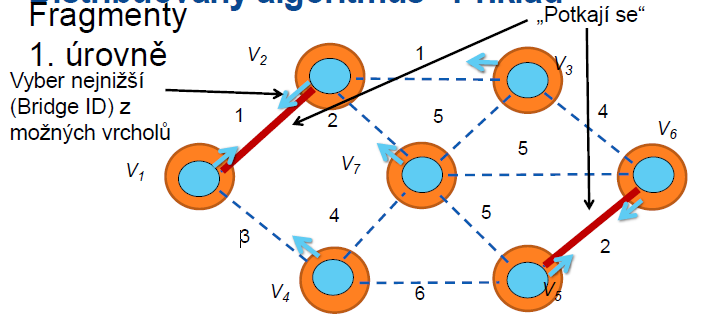
\includegraphics[scale=0.5]{BPC-TIN/images/distributed1.PNG}
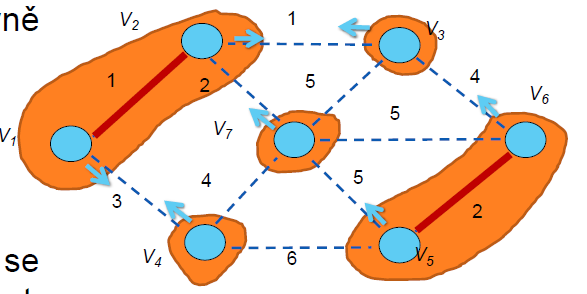
\includegraphics[scale=0.5]{BPC-TIN/images/distributed2.PNG}
\end{center}

\begin{Large}\vspace{0,5cm} \textbf{Slepé prohledávání}
\end{Large}

\textbf{BFS}\,--\,využívá frontu do kterého prvně vloží vstupní vrchol. Z tohoto vrcholu se vezmou všichni sousedé a vloží se do fronty, z které se bere postupně a jejich sousedé se přidávají do fronty. Při tomto se každá už navštívený vrchol ukládá do nějakého pole/seznamu navštívených abychom ho nenavštěvovali znovu.

Video \url{https://www.youtube.com/watch?v=oDqjPvD54Ss}

\textbf{DFS}\,--\,pracuje na principu, že prozkoumává prvně vrchol na jednu stranu a v ní pokračuje dokud nedojde na konec nebo nedorazí do už navštíveného vrcholu. Využívá zásobník.

Video \url{https://youtu.be/pcKY4hjDrxk?t=279}

BFS vs DFS rozdíl je že DFS je méně paměťově náročné ale BFS je optimální.

\textbf{DLS}\,--\,vychází z DFS ale je omezen na maximální hloubku.

\textbf{IDLS}\,--\,iterativní prohledávaní do hloubky. Vychází z DFS ale v každé iteraci se prohledává jen o hloubku níž. Video \url{https://www.youtube.com/watch?v=Y85ECk_H3h4}

\textbf{Dijkstrův algoritmus}\,--\,využívá prioritní frontu a nějaký seznam navštívených vrcholů. Z prvního vrcholu se přidají všechny soudní vrcholy z jejich hodnotou hrany do prioritní fonty. Z prioritní fronty se vždy vezme nejmenší prvek. Z nejnižšího vrcholu se prozkoumají znovu sousedé ale tentokrát se nepoužije pouze vzdálenost mezi nimi ale přičte se už i vzdálenost k aktuálnímu vrcholu. Tak se bere dokud se nedorazí k cílovému vrcholu.

Video \url{https://www.youtube.com/watch?v=GazC3A4OQTE}


\begin{Large}\vspace{0,5cm} \textbf{Informovaná metoda}
\end{Large}

\textbf{A*}\,--\,využívá prioritní frontu a nějaký seznam navštívených vrcholů. Každému z vrcholu přidělíme vzdálenost od cíle. Postupuje se stejně jako u Dijktrova algoritmu ale s tím rozdílem že sčítáme vzdálenost + hodnotu hrany. Dle této sečtené hodnoty vybíráme další navštívený prvek z prioritní fronty.

Video \url{https://www.youtube.com/watch?v=ySN5Wnu88nE}







\newpage
\section{Evoluční algoritmy. Genetické algoritmy, genetické programování. Pojmy populace, mutace, křížení, chromozom. Princip evolučních algoritmů.}

Optimalizace a jejími úlohami se setkáváme při řešení praktických úloh, při kterých hledáme to nejlepší možné řešení. O nejlepším řešení se rozhodujeme dle parametrů.

\begin{Large}\vspace{0,5cm} \textbf{Evoluční algoritmy}
\end{Large}

Je jeden ze způsobů optimalizace. Byli vytvořeny, aby sjednotili optimalizační metody co využívají \uv{evoluční} principy. Evoluční algoritmy zastřešují pod sebou řadu přístupů využívající modely biologické evoluce. Tyto modely jsou přirozený výběr (výběr silnějšího jedince, podle fitness funkce), náhodný genetický drift (mutace, decimuje jedince s vysokou fitness) a reprodukční proces (křížení jedinců). Spadají zde přístupy jako genetické algoritmy, genetické programovaní, evoluční strategie, evoluční programovaní.

Obecný evoluční algoritmus funguje zjednodušeně, že prvně máme nějakou základní populaci. S této populace uděláme výběr jedinců. Vybrané jedince zkřížíme. Tyto jedinci následně zmutují a vytvoří se nová populace. Tyto kroky se opakují v N iteracích. Kde ukončení stanovuje předem stanovený počet iterací, dosažení požadovaného jedince popřípadě minimální změnou fitness populace po několik iterací.

\begin{Large}\vspace{0,5cm} \textbf{Genetické algoritmy}
\end{Large}

Genetické algoritmy jsou založeny na Darwinově myšlence že přežije nejsilnější. Využívá metody křížení, mutace a selekce.

TODO Kódování řetězci má také svou analogii v gentice, kdy v podstatě řetězce odpovídají chromozómům, jednotlivé pozice v řetězci jednotlivým genům a konkrétní hodnoty na těchto pozicích pak alelám.

Genetické algoritmy pracují tak že prvně vyberou nějakou populaci přípustných řešení. Abychom s nimi mohly pracovat musíme je převést do řetězce/pole. Poté přichází na řadu výběr jedinců, kteří se budou podílet na nové generaci. Vetšinou to probíhá tak, že ohodnotíme každého jedince pomocí fitness funkce a na základě tohoto parametru vybereme nejvhodnější kandidáty (metod výběru je více). Tito vybraní jedinci se mezi sebou kříží. Nakonec každý kandidát mutuje. 

Výhody GA jsou že nevyžadují žádné speciální znalosti o cílové funkci, jsou odolné, aby nesklouzli do lokálního optima.

Nevýhody GA jsou že mají problém s nalezením přesného optima, vyžadují velké množství vyhodnocování cílové funkce.

\begin{Large}\vspace{0,5cm} \textbf{Genetické programování}
\end{Large}

Hledá samotnou funkci a ne její parametry. Oproti GA se liší v reprezentaci jedinců. V GP jsou jedinci vytvořeni stromem s proměnlivou délkou chromozomu. Zjednodušeně je to převedení GA do programovacích jazyků.

\begin{Large}\vspace{0,5cm} \textbf{Základní pojmy}
\end{Large}

\textbf{Populace}\,--\,je množina jedinců o určité velikosti, z které následně vybíráme jedince na operace (křížení, mutace atd) při evoluci. Konkrétní populace se nazývá genotyp. 

\textbf{Jednice}\,--\,člen populace, který je definován jedním chromozomem.

\textbf{Chromozom}\,--\,je to řetězec tvořený geny, který má za úkol se odlišit od zbytku populace (DNA). Lze ho kódovat např. binárně, reálnými čísly, znaky, objekty(instance třídy v programovaní).

\textbf{Gen}\,--\,na i-té pozici reprezentuje stejnou charakteristiku v každém jedinci.

\textbf{Alela}\,--\,hodnota které může nabývat gen (např 0, 1).

\textbf{Fitness funkce}\,--\,kvantitativně vyjadřuje kvalitu každého řešení. Např. dosažení požadované přesnosti algoritmu, množství času potřebné pro výpočet algoritmu, množství chyb mezi skutečným a požadovaným výstupem.

Více druhů metod vytvoření fitness funkce (Hrubá, standardizovaná, přizpůsobená, normalizovaná)

\textbf{Selekce ruletový výběr varianta 1}\,--\,pravděpodobnost výběru závisí na kvalitě jedince (kolik místa na ruletě zabírá). Pokud jedince bude převyšovat ostatní o hodně nové populace budou tvořeny jeho geny, k tomu se dají použít techniky potlačení/podpory.

\textbf{Selekce ruletový výběr varianta 2}\,--\,jedinci jsou seřazeni vzestupně podle hodnoty fitness a velikost místa je určena rovnicí. Tímto se potlačují nadprůměrní jedinci, kteří by negativně ovlivňovali další generace.

\textbf{Selekce turnajový výběr}\,--\,náhodně se vybere n jedinců a postupným porovnáváním je vybrán nejlepší.

\begin{Large}\vspace{0,5cm} \textbf{Metody křížené}
\end{Large}

\textbf{Elitářství}\,--\,zaručuje monotonní hodnotu fitness nejlepšího jedince, předchází ztrátě nejlepšího řešení.

\begin{center}
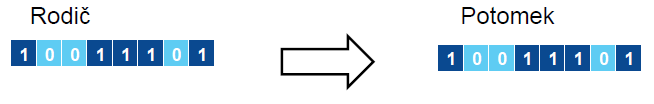
\includegraphics[scale=0.7]{BPC-TIN/images/elita.PNG}
\end{center}

\textbf{Křížení n-bodové}\,--\,dělí se v n bodech a vymění se mezi sebou.

\begin{center}
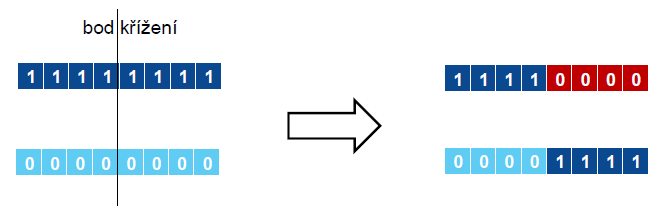
\includegraphics[scale=0.55]{BPC-TIN/images/1bod.PNG}
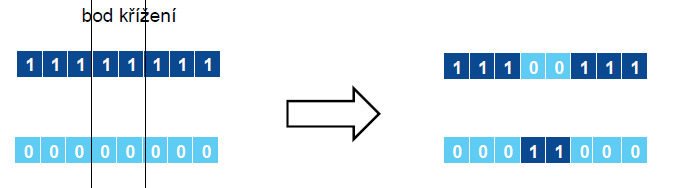
\includegraphics[scale=0.55]{BPC-TIN/images/2bod.PNG}

\end{center}

\textbf{Křížení uniformní}\,--\,rozvrací kód chromozomu, dobrý pro vnešení diverzity.

\begin{center}
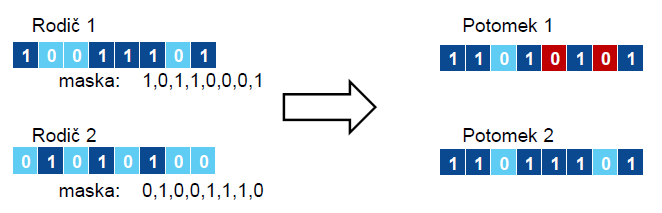
\includegraphics[scale=0.7]{BPC-TIN/images/uniform.PNG}
\end{center}

\textbf{Mutace}\,--\,Aplikuje se s malou pravděpodobností, důležitá pokud máme málo jedinců.

\begin{center}
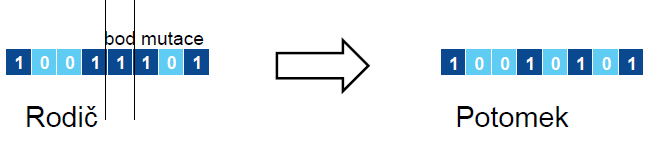
\includegraphics[scale=0.7]{BPC-TIN/images/mutace.PNG}
\end{center}